\en

\section{Tool architecture}
\label{subsec:architecture}

The Setup step consists of the Function Breaker and the Code Duplication Finder. The pipeline of this step works as follows: the Function Parser receives the codebase the user is interested in, extracts the functions of the codebase along with metadata, and creates a new temporary codebase where the functions extracted become new code files. The Code Duplication Finder iterates over every pair of files in the temporary codebase, checks if they are code clones, and, if so, saves them in the Code Duplication Database, which is a text file that stores every code duplication as a triple \textbf{<function1,function2,similarity>}, where \textbf{function1} and \textbf{function2} are the functions that are duplicates of each other, and \textbf{similarity} is the metric given by the code duplication detection method utilized, which in our case is the cosine similarity explained in Section \ref{sec:similarity}. Finally, the Query Responder consumes the temporary codebase and the Code Duplication Database to extract duplicated functions-related information per user request. Figure \ref{fig:diagram} illustrates the tool pipeline. An explanation of how each component works is provided in this section.

\begin{figure}
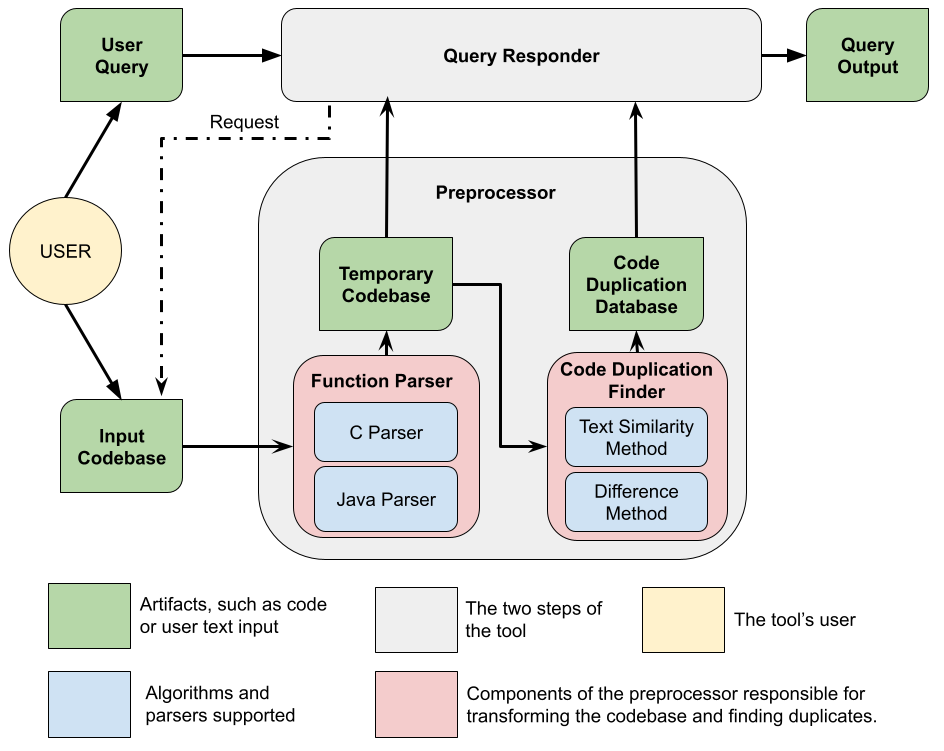
\includegraphics[scale=0.5]{diagrama_mestrado}
\caption{Architecture diagram demonstrating the relationship between the tool components.}
\label{fig:diagram}
\end{figure}

\subsection{Input codebase}

The input codebase is a folder on the machine running the tool. All files in the codebase that are not source code files from a programming language supported by the tool are ignored. The tool validates support for a source file by analyzing its file extension.

\subsection{Function Parser}

The Function Parser receives the input codebase and transforms it into the temporary codebase. The Function Parser iterates through every source code file from the programming language it supports and uses a specific programming language function extractor to extract every function in the file. For each function extracted, two new source code files and a metadata file are created in the temporary codebase, represented by the pair \textbf{<file name, function name>}, the source code file of the function, and the proper function. The first new source code file contains the function's body from the function it represents, while the other new source code file contains the function's signature. The metadata file contains additional relevant information about the function, such as the function name, the line where the function signature starts in the source code file, and the line where the function's body ends in the source code file. The programming languages supported at the moment are C and Java. Figure \ref{fig:transform} illustrates an example of a function transformation into the temporary codebase.

\begin{figure}
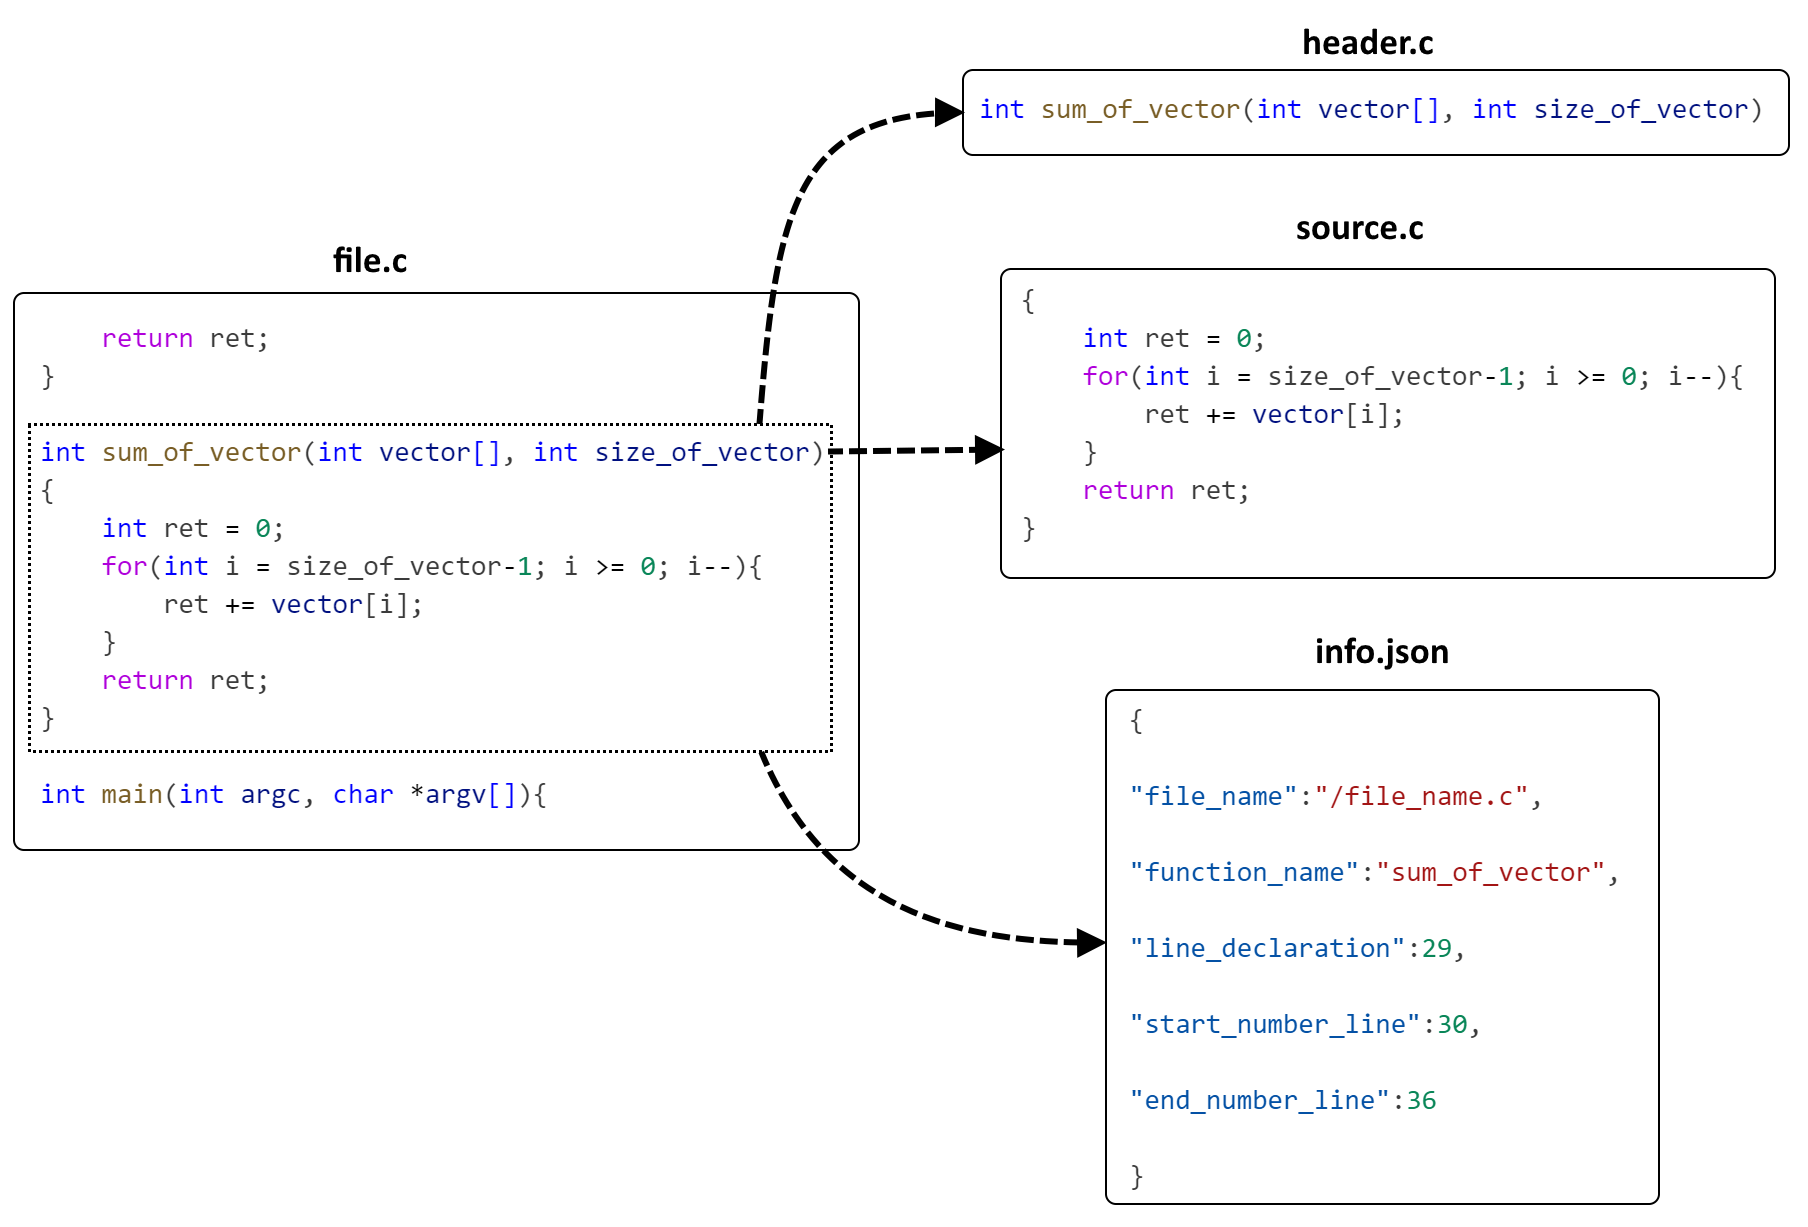
\includegraphics[scale=0.3]{example_function_parser/example_parser}
\caption{Transformation of a function into the temporary codebase}
\label{fig:transform}
\end{figure}

Regarding the programming language's function extractor, we approached this problem so that anyone comfortable with a language can adapt our approach to their specific programming language. Usually, code blocks can be easily extracted from source code files, independently if the code blocks are defined by curly brackets or by indentation, and it is possible to infer if they represent a function's body given their depth in the code context and a few lines before the start of the code block. We followed this approach to implement the function extractor for the supported languages. As an alternative approach, we can build the syntax tree \citep{compiler} of the programming language and use it to extract the functions, which is a more complex task than our approach. For the programming languages that we support, we implemented them as follows:

\begin{itemize}
	\item \textbf{C}: Given a source code file, we extract every code block from it, maintaining the depth of the code block in the code context and some of the code lines before the definition of the code block. According to the C programming language's grammar, functions are defined in a global context at depth 0. There are other elements with the same depth as functions, and we differentiate them by analyzing if the first non-empty character before the curly brackets of the code block is a closing parenthesis. This pattern uniquely identifies functions within C code.

	\item \textbf{Java}:  Given a source code file, we extract every code block from it, maintaining the depth of the code block in the code context and some of the code lines before the definition of the code block. According to Java's grammar, functions are defined inside classes. Functions can exist at different depths, as Java accepts inner classes. We differentiate functions from other elements by analyzing if the first non-empty character before the curly brackets of the code block is a closing parenthesis. A challenge with this approach in Java is that other elements, such as for-loops, can follow this pattern, necessitating additional filters. We chose to analyze functions at depth 1, which ignores any other element that is a code block and has a parenthesis as the first non-empty character before the curly brackets. This choice means the extractor does not find functions declared inside inner classes, but this limitation is not an issue in this work, as there are no inner classes in BigCloneBench \citep{bigclonebench}, the only Java codebase explored in this work.
\end{itemize}

\subsection{Temporary codebase}

The temporary codebase is a transformation of the input codebase performed by the Function Parser. Each function in the input codebase is represented in the temporary codebase as three files. Descriptions of these files are provided below, with examples shown in Figure \ref{fig:transform}.

\begin{itemize}
	\item \textbf{Header file}: This file contains the signature of the function it represents.
	\item \textbf{Source file}: This file contains the body of the function it represents.
	\item \textbf{Info file}: This file contains metadata about the function, including the function name, the file that contains the function, the file's relative path to the input codebase, the line where the function's signature starts, the line where the function body begins, the line where the function's body ends, and whether there is a line break between the end of the function's signature and the start of the function's body.
\end{itemize}

\subsection{Code Duplication Finder}

The Code Duplication Finder iterates through every pair of source code files in the temporary codebase, representing functions from the input codebase. For each pair of files, we execute a code duplication detection method that computes a metric measuring how similar the pair of files is, which we refer to as similarity. If the similarity is greater than or equal to the minimum similarity threshold (a parameter provided by the user during the Setup step), we store this pair of functions along with its similarity in the Code Duplication Database.

For the code duplication detection method, we treat the source code files as text and apply the TF-IDF vector embedding method implemented by the Gensim library \citep{gensim}, then compute cosine similarity as the similarity metric. This method was chosen for its claimed performance, programming language independence, and the fact that it does not require compilable code, which is expected in the temporary codebase, as it does not contain complete code artifacts. \cite{platistool} implemented this code duplication detection method and released it under the MIT license \citep{mitlicense}. We adapted his implementation to fit our tool's expected input and output formats. Switching the duplication detection method is feasible, similar to how we adapted Plates' implementation.

\subsection{Code Duplication Database}

The Code Duplication Database is a text file that contains the duplicated pairs of functions found by the Code Duplication Finder. The first line of the file specifies the number of duplicated pairs. Following this, each line lists a duplicated pair, including the paths of the functions in the temporary codebase and the similarity metric of the pair.

\subsection{Setup step}
\label{subsec:setup}

The Setup step is a procedure executed by the user once per codebase. The Setup step takes the input codebase and a minimum similarity metric value for function pairs considered duplicates. It then runs the Function Parser and the Code Duplication Finder to create a temporary codebase and the Code Duplication Database. Setting a minimum similarity metric reduces the Code Duplication Database size, optimizing memory usage and the computational cost of the Query Responder step. For example, if this parameter does not exist and we work with a codebase of $10000$ functions, each with a 50-character relative path and function name, the Code Duplication Database would reach approximately $5000^2 \times 50 ~= 5$ gigabytes. As most function pairs are unlikely to be duplicated in large codebases, this file size can be significantly reduced.

\subsection{Query Responder step}

The Query Responder step is the component the user executes multiple times to consult information about duplicated functions in a codebase processed by the Setup step. The Query Responder step utilizes the temporary codebase and the Code Duplication Database as inputs to answer the user's request, such as querying the total number of duplicated functions in a specific input codebase or listing duplicated functions above a certain similarity threshold. This component was developed to be extensible, allowing other queries to be easily added. Currently, the Query Responder step supports the following queries:

\begin{itemize}
	\item Number of duplicated functions above a similarity threshold.
	\item Number of duplicated functions equal or above a similarity threshold.
	\item List of duplicated functions above a similarity threshold.
	\item List of duplicated functions equal to or above a similarity threshold.
\end{itemize}
